\documentclass[11pt]{article}
\usepackage{mathtools}
\usepackage{mdframed}
\usepackage{fullpage}
\usepackage{amsfonts}
\usepackage{array}
\usepackage{tikz}
\usetikzlibrary{automata, positioning}



%edit this for each class
\newcommand\name{John Vincent}
\newcommand\classname{Com S 311}
\newcommand\assignment{Homework 3}



\newcounter{excounter}
\setcounter{excounter}{1}
\newcommand\question[2]{\vskip 1em  \noindent\textbf{\arabic{excounter}\addtocounter{excounter}{1}.} \emph{#1} \noindent#2}


% You can also erase this if you do not have package fancyhdr
% Fancy footnote.........
\usepackage{fancyhdr}  %% If it does not work with your latex installation, you may just delete this...
\pagestyle{fancy}
\usepackage{lastpage}
\rfoot{\name, page \thepage/\pageref{LastPage}}
\cfoot{}
\rhead{}
\lhead{}
\renewcommand{\headrulewidth}{0pt}
\renewcommand{\footrulewidth}{0pt}
\DeclarePairedDelimiter\ceil{\lceil}{\rceil}
\DeclarePairedDelimiter\floor{\lfloor}{\rfloor}

\newenvironment{hashtable}[1][]
  {\begin{center}\begin{tabular}[#1]{
     @{}
     > {\small} r <{\normalsize~\rlap{\fbox{\strut~~}}$~~\rightarrow$~}
     @{} l @{}}}
  {\end{tabular}\end{center}}


\begin{document}


  {\bf \classname \hspace{1cm} \assignment\hfill \name}
  \vskip 2em


  \question{}\\
  \indent a)\\
  \begin{center}
    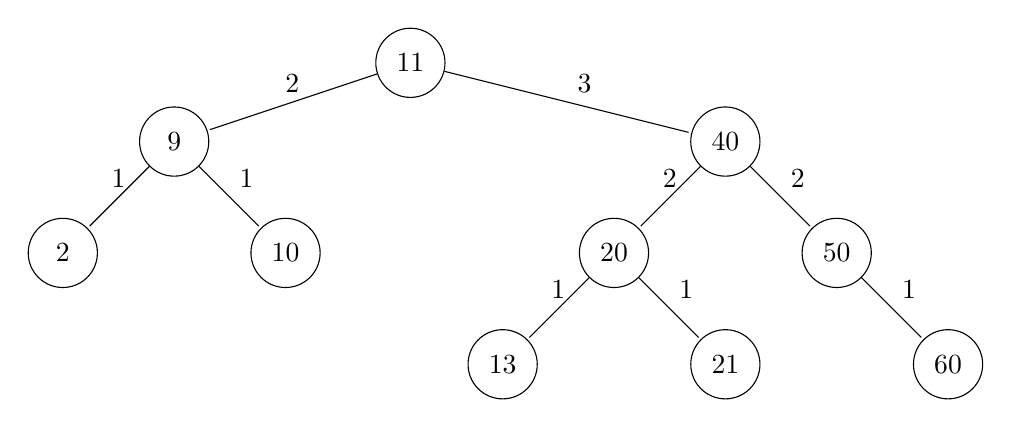
\begin{tikzpicture}[shorten >=1pt,node distance=2cm,on grid,auto]
      \node[state] (q_0) {$11$};
      \node[state] (q_1) [below right = 1cm and 4cm of q_0] {$40$};
      \node[state] (q_2) [below left of= q_1] {$20$};
      \node[state] (q_3) [below left of=q_2] {$13$};
      \node[state] (q_4) [below right of=q_2] {$21$};
      \node[state] (q_5) [below right of=q_1] {$50$};
      \node[state] (q_6) [below right of=q_5] {$60$};
      \node[state] (q_7) [below left=1cm and 3cm of q_0] {$9$};
      \node[state] (q_8) [below left of=q_7] {$2$};
      \node[state] (q_9) [below right of=q_7] {$10$};

      \path (q_0) edge node {3} (q_1)
            (q_0) edge node [above] {2} (q_7);
      \path (q_1) edge node [above] {2} (q_2)
            (q_1) edge node {2} (q_5);
      \path (q_2) edge node [above] {1} (q_3)
            (q_2) edge node {1} (q_4);
      \path (q_5) edge node {1} (q_6);
      \path (q_7) edge node [above] {1} (q_8)
            (q_7) edge node {1} (q_9);
    \end{tikzpicture}
  \end{center}

  \indent b) the tree is already balanced as all left and right children differ in
  height by at most 1.

  \indent c)
  \begin{hashtable}
    0 & 11 $\rightarrow$ 21\\
    1 & 9\\
    2 & 2\\
    3 & 40 $\rightarrow$ 20 $\rightarrow$ 50 $\rightarrow$ 60 $\rightarrow$ 10\\
    4 & 13
  \end{hashtable}

  \question{}\\
  \null\hspace{.5cm}a)
  \begin{quote}
    since $T$ is perfectly balanced and full we known that any node at height $h$ has $\frac{2^h -2}{2}$ nodes on the left and right side of it.
    The right child $R$ of the root would then have $h_R = \ell-1$. The number of,
    children $c$ on its right side can be calculated by
    \begin{align*}
      c &= \frac{2^{\ell-1}-2}{2}\\
        &= \frac{2^{\ell-1}}{2}-\frac{2}{2}\\
        &= 2^{\ell-2}-1
    \end{align*}
    so the right child of the root is always smaller than $2^{\ell-2}-1$ elements making the algorithm selecting the right child of the root if one exist,
    otherwise selecting the root. This has time complexity $O(1)$ because it is not dependant on the size of the tree in any way. We know this is correct because
    the element we are looking for is smaller than a little less than $\frac{1}{4}$ the elements in $T$.
    \begin{align*}
      2^{x-2} -1   &\approx \frac{2^x-1}{4}\\
      4(\frac{2^{x}}{4} -1) &\approx 2^{x}-1\\
      2^{x} - 4  &\approx 2^x-1
    \end{align*}
    The right child of the root is smaller than its right child which is almost $\frac{1}{4}$ the elements in $T$.
  \end{quote}
  \null\hspace{.5cm}b)
  \begin{center}
    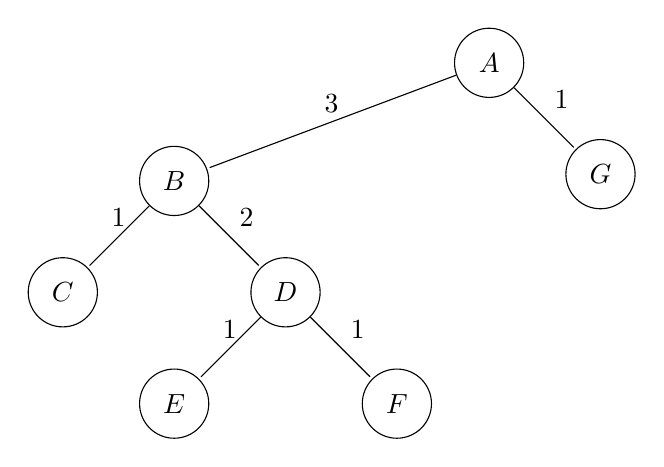
\begin{tikzpicture}[shorten >=1pt,node distance=2cm,on grid,auto]
      \node[state] (q_0) {$A$};
      \node[state] (q_1) [below left = 1.5cm and 4cm of q_0] {$B$};
      \node[state] (q_2) [below left of= q_1] {$C$};
      \node[state] (q_3) [below right of=q_1] {$D$};
      \node[state] (q_4) [below left of=q_3] {$E$};
      \node[state] (q_5) [below right of=q_3] {$F$};
      \node[state] (q_6) [below right of=q_0] {$G$};

      \path (q_0) edge node {1} (q_6)
            (q_0) edge node [above] {3} (q_1);
      \path (q_1) edge node [above] {1} (q_2)
            (q_1) edge node {2} (q_3);
      \path (q_3) edge node [above] {1} (q_4)
            (q_3) edge node {1} (q_5);
    \end{tikzpicture}
  \end{center}
  \begin{center}
    \begin{tikzpicture}[shorten >=1pt,node distance=2cm,on grid,auto]
      \node[state] (q_0) {$A$};
      \node[state] (q_3) [below left = 1.5cm and 4cm of q_0] {$D$};
      \node[state] (q_1) [below left of= q_3] {$B$};
      \node[state] (q_2) [below left of= q_1] {$C$};
      \node[state] (q_4) [below right of=q_1] {$E$};
      \node[state] (q_5) [below right of=q_3] {$F$};
      \node[state] (q_6) [below right of=q_0] {$G$};

      \path (q_0) edge node {1} (q_6)
            (q_0) edge node [above] {3} (q_3);
      \path (q_1) edge node [above] {1} (q_2)
            (q_1) edge node {1} (q_4);
      \path (q_3) edge node [above] {2} (q_1)
            (q_3) edge node {1} (q_5);
    \end{tikzpicture}
  \end{center}
  \begin{center}
    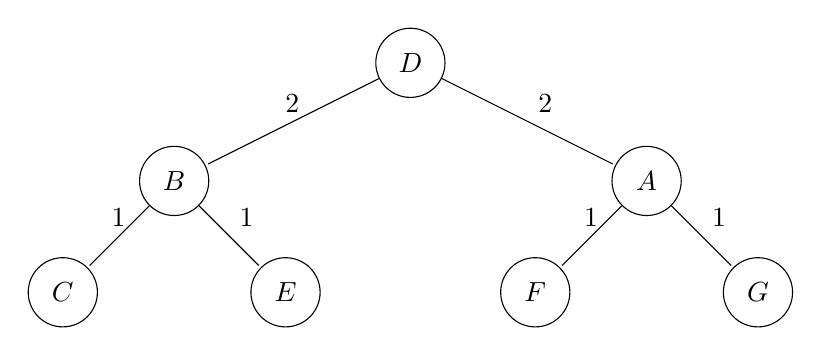
\begin{tikzpicture}[shorten >=1pt,node distance=2cm,on grid,auto]
      \node[state] (q_3) {$D$};
      \node[state] (q_0) [below right = 1.5cm and 3cm of q_3] {$A$};
      \node[state] (q_1) [below left = 1.5cm and 3cm of q_3] {$B$};
      \node[state] (q_2) [below left of= q_1] {$C$};
      \node[state] (q_4) [below right of=q_1] {$E$};
      \node[state] (q_5) [below left of=q_0] {$F$};
      \node[state] (q_6) [below right of=q_0] {$G$};

      \path (q_0) edge node {1} (q_6)
            (q_0) edge node [above] {1} (q_5);
      \path (q_1) edge node [above] {1} (q_2)
            (q_1) edge node {1} (q_4);
      \path (q_3) edge node [above] {2} (q_1)
            (q_3) edge node {2} (q_0);
    \end{tikzpicture}\\
    the balance factors of A,B, and D are  0.
  \end{center}

  \question{}\\
  \null\hspace{.5cm}a)
  \begin{quote}
    To construct a B Tree from an array where all the elements of the array are leaves in the tree, you would first construct a new array $A_1$ of size
    $\floor{n/2}$, where $A_1[i] = \frac{A[i*2]+A[i*2-1]}{2}$. $A_1$ will be the array of parents to $A$.
    you then repeat the proccess until you create an array of size $1$ each array being the direct parent of the two elements used to calculate its value.
    The runtime can be expressed by the function $F$
    \[F(n)= \sum_{i=0}^{log_2n}\frac{n}{2^i} = n \sum_{i=0}^{log_2n}\frac{1}{2^i}\implies O(F) = O(n\log n)\]
  \end{quote}
  \null\hspace{.5cm}b)
  \begin{quote}
    
  \end{quote}

\end{document}
